\documentclass[11pt]{article}
\usepackage[T1]{fontenc}
\usepackage{lmodern}
\usepackage[letterpaper,margin=1in]{geometry}
\usepackage{microtype}
\usepackage{amsmath,amssymb}
\usepackage{graphicx,booktabs}
\usepackage[numbers,sort&compress]{natbib}
\usepackage[hidelinks]{hyperref}

\title{Learning Logistic Growth with Neural ODEs:\\
Comparing a Learned Model with an Exact Solution}
\author{Sebastian Chegini}
\date{}

\begin{document}
\maketitle

\begin{abstract}
A Neural Ordinary Differential Equation (Neural ODE) uses a neural network to
represent a system's rate of change. This project investigates how well such a
model can learn logistic growth from samples of a single solution. We first
derive the exact solution using the Bernoulli substitution, then use it to
generate 100 noise-free training points. A small neural network represents the
growth rate, and a fourth-order Runge--Kutta solver produces the predicted
population. In the reference run, the learned trajectory has a root-mean-square
error of approximately $0.20$ population units over the training points, but
eventually exceeds the true carrying capacity. The same overshoot occurs in
ten runs with different random initializations. Examining the learned growth
rate shows that the models do not recover the equilibrium at the carrying
capacity. For this experiment, agreement with the observed growth curve does
not guarantee agreement with the system's long-term behavior.
\end{abstract}

\section{Introduction}

Residual networks update a hidden state by adding a learned correction to its
current value \cite{he2016deep}. An update of the form
\[
 h_{k+1}=h_k+\Delta t\,f_\theta(h_k)
\]
resembles a forward Euler step for a differential equation. This connection
motivates Neural ODEs, which describe the evolution of a state through a
neural network representing its derivative \cite{chen2018neural}:
\begin{equation}
 \frac{dy}{dt}=f_\theta(y(t),t), \qquad y(t_0)=y_0.
 \label{eq:node}
\end{equation}
The prediction at a later time is obtained by solving this initial value
problem numerically. Rather than directly predicting a population from a time
input, the network in this project learns a rule for how the population changes.

The main question is how accurately this approach reproduces a known growth
model. Logistic growth is a useful example because the solution can be found
analytically with techniques from an introductory differential equations
course. We can therefore compare the learned trajectory with an exact solution,
and also compare the learned rate of change with the differential equation
that generated the data.

We first derive the logistic solution using the Bernoulli substitution. We then
train a Neural ODE on samples from this solution and examine both its prediction
error and its behavior near the carrying capacity. The data are synthetic;
bacterial growth provides the motivation for the example, rather than a source
of experimental measurements.

\section{The logistic growth model}

\subsection{Model and parameters}

Let $y(t)$ denote population size in arbitrary population units, with time
measured in hours. With unlimited resources, the equation $y'=ry$ describes
exponential growth. The logistic model adds a factor that reduces the growth
rate as the population approaches the carrying capacity $K$:
\begin{equation}
 \frac{dy}{dt}=ry\left(1-\frac{y}{K}\right),\qquad y(0)=y_0.
 \label{eq:logistic}
\end{equation}
Here $r>0$ is the intrinsic growth rate and $K>0$ is the population that the
environment can sustain. When $y$ is small relative to $K$, the growth is
approximately exponential. As $y$ approaches $K$, the growth rate approaches
zero. In this example we use
\[
 r=0.5\,\mathrm{h}^{-1},\qquad K=10,\qquad y_0=0.1.
\]
These are scaled population units, so the initial value does not mean a
fraction of an individual bacterium.

\subsection{Solution using the Bernoulli substitution}

A Bernoulli equation has the form
\[
 y'+P(t)y=Q(t)y^n.
\]
For $n\ne0,1$, the substitution $z=y^{1-n}$ reduces the equation to a linear
equation on an interval where the powers and the substitution are defined.
Expanding Equation~\eqref{eq:logistic} gives
\[
 y'-ry=-\frac{r}{K}y^2,
\]
so $P(t)=-r$, $Q(t)=-r/K$, and $n=2$. For the positive population considered
here, we set $z=y^{-1}$. Since $z'=-y^{-2}y'$, multiplying the equation by
$-y^{-2}$ gives
\[
 -y^{-2}y'+ry^{-1}=\frac{r}{K},
 \qquad\text{or}\qquad z'+rz=\frac{r}{K}.
\]
This is a first-order linear equation with integrating factor $e^{rt}$.
Multiplication by this factor gives
\[
 e^{rt}z'+re^{rt}z=\frac{r}{K}e^{rt},
 \qquad
 \frac{d}{dt}\left(e^{rt}z\right)=\frac{r}{K}e^{rt}.
\]
Integrating both sides, we obtain
\[
 e^{rt}z=\frac{1}{K}e^{rt}+C,
 \qquad z=\frac{1}{K}+Ce^{-rt}.
\]
Substituting back for $y$ gives
\[
 y(t)=\frac{K}{1+CKe^{-rt}}.
\]
Writing $A=CK$ and applying $y(0)=y_0$ yields
\[
 y_0=\frac{K}{1+A},\qquad A=\frac{K-y_0}{y_0}.
\]
For the chosen parameters, $A=99$, so the exact solution is
\begin{equation}
 y(t)=\frac{10}{1+99e^{-0.5t}}.
 \label{eq:solution}
\end{equation}
For example, the predicted population after ten hours is
\[
 y(10)=\frac{10}{1+99e^{-5}}\approx5.9986.
\]

\subsection{Behavior to compare with the learned model}

Equation~\eqref{eq:logistic} has equilibrium solutions $y=0$ and $y=K$.
For $0<y<K$, the derivative is positive; for $y>K$, it is negative.
Thus a population starting between $0$ and $K$ grows toward $K$.
Equation~\eqref{eq:solution} also shows that this population remains strictly
below $K$ at every finite time. In particular, $y(20)\approx9.9553$.

The growth rate is greatest at $y=K/2$. To see this, differentiate the
right-hand side $f(y)=ry(1-y/K)$:
\[
 f'(y)=r\left(1-\frac{2y}{K}\right).
\]
The maximum occurs at $y=K/2=5$, where $f(y)=rK/4=1.25$ population units per
hour. The trajectory reaches this value at $t=2\ln99\approx9.19$ hours.
These properties let us assess more than whether two curves look similar.

\section{Neural ODE construction and training}

\subsection{Data and network}

The training data consist of 100 equally spaced samples from
Equation~\eqref{eq:solution} over $0\le t\le20$:
\[
 t_i=\frac{20i}{99},\qquad y_i=y(t_i),\qquad i=0,\ldots,99.
\]
The data contain no added noise. All 100 points are used for training and for
the reported trajectory errors.

The network has one input, two hidden layers of 50 units each with hyperbolic
tangent activations, and one output:
\[
 1\longrightarrow50\longrightarrow50\longrightarrow1.
\]
Its input is the current population, and its output is the predicted rate of
change. Although Equation~\eqref{eq:node} allows explicit time dependence,
this implementation does not use time as a network input. The learned equation
is therefore autonomous:
\[
 \frac{d\hat y}{dt}=f_\theta(\hat y),\qquad \hat y(0)=0.1.
\]
The initial condition is supplied, but the network is not given $r$, $K$, or
the logistic formula. Those quantities are used to generate the target data.

\subsection{Numerical solution and optimization}

We solve the learned equation using the classical fourth-order Runge--Kutta
method (RK4). For this autonomous model, one step is
\begin{align*}
 k_1&=f_\theta(\hat y_n),&
 k_2&=f_\theta(\hat y_n+hk_1/2),\\
 k_3&=f_\theta(\hat y_n+hk_2/2),&
 k_4&=f_\theta(\hat y_n+hk_3),\\
 \hat y_{n+1}&=\hat y_n+\frac{h}{6}(k_1+2k_2+2k_3+k_4).
\end{align*}
The step size is $h=20/99\approx0.202$ hours, matching the sampling interval.
Each predicted trajectory requires 99 steps and 396 evaluations of the network.

Training minimizes the mean squared error
\begin{equation}
 \mathcal L(\theta)=\frac{1}{100}\sum_{i=0}^{99}
 \left(\hat y_i(\theta)-y_i\right)^2.
 \label{eq:loss}
\end{equation}
We use Adam \cite{kingma2015adam} with a learning rate of $0.01$ for 1,000
iterations. Gradients are computed by backpropagating through the RK4 steps.
The experiment is repeated with random seeds 0 through 9, using the default
PyTorch network initialization. Seed 0 serves as the reference run shown in
Figure~\ref{fig:fit}. The supplied implementation uses a single CPU thread;
the saved results report PyTorch 2.10.0.

For evaluation, we report the root-mean-square error (RMSE) and maximum
absolute error at the training points. A second integration uses 20 smaller
RK4 steps per sampling interval to check sensitivity to the integration step
and obtain predictions between samples. We also integrate to $t=100$ hours
and search for sign changes of $f_\theta(y)$ on a grid of 30,001 points over
$0\le y\le30$. Linear interpolation between neighboring grid points gives
approximate equilibrium locations. This search detects sign-changing roots;
it does not rule out every possible zero of the learned field.

\section{Results}

\subsection{Reference run}

In the reference run, the final mean squared error is approximately $0.0385$,
corresponding to an RMSE of $0.196$ population units. The maximum absolute
error is $0.334$. Figure~\ref{fig:fit}(a) shows that the learned trajectory
follows the main shape of the exact solution, including its transition from
rapid growth toward saturation.

\begin{figure}[tbp]
 \centering
 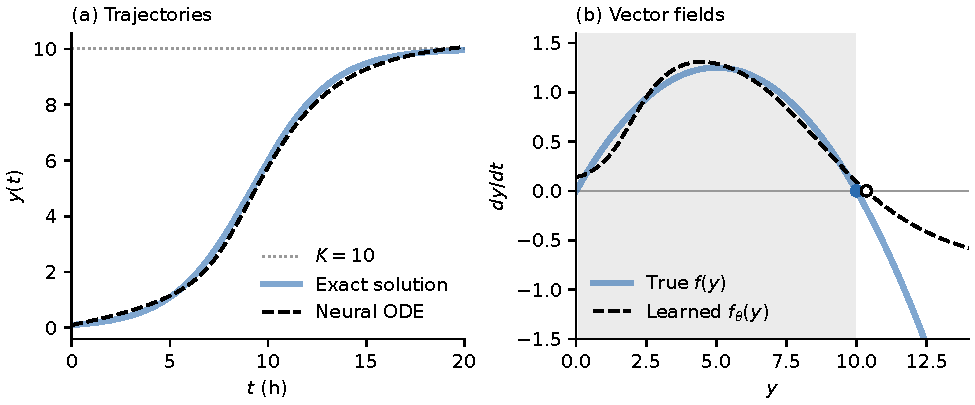
\includegraphics[width=\linewidth]{figures/neural-ode-fit.pdf}
 \caption{Reference run (seed 0). Left: the exact logistic solution and the
 learned trajectory over the training interval. The horizontal dotted line
 marks $K=10$. Right: the true and learned growth rates. The shaded region
 shows the range of population values in the training data. The filled and
 open circles mark the true equilibrium at $K$ and the numerically located
 learned equilibrium near $10.35$, respectively.}
 \label{fig:fit}
\end{figure}

At $t=10$ hours, the learned model predicts $\hat y(10)\approx5.765$, compared
with the exact value $5.999$, a relative error of approximately $3.9\%$.
Near the end of the interval, the difference is qualitative as well as
numerical. The learned trajectory crosses $K=10$ at approximately $19.13$
hours and reaches $\hat y(20)\approx10.072$. The exact logistic trajectory
never reaches $K$ in finite time.

The learned growth rate explains this overshoot. At the true carrying
capacity, $f_\theta(10)\approx0.092>0$, so the learned equation still predicts
growth. Its growth rate changes from positive to negative near $y=10.35$,
indicating a stable equilibrium above the true carrying capacity. The
integration to $t=100$ approaches this value. At the other true equilibrium,
$f_\theta(0)\approx0.141$, so the network also fails to recover the zero
population equilibrium.

Reducing the integration step changes the reference trajectory at the sample
times by at most $5.8\times10^{-6}$ population units. This comparison suggests
that the observed overshoot is not caused by the coarse integration step.
It is a numerical consistency check, rather than a rigorous error bound
relative to the exact solution of the learned equation.

\subsection{Different random initializations}

Table~\ref{tab:runs} summarizes the ten runs. Their RMSE values range from
$0.118$ to $0.348$, and every prediction at $t=10$ is within $4\%$ of the
exact value. However, every run crosses $K$ before $t=20$, and every learned
field is positive at both $y=0$ and $y=10$.

\begin{table}[tbp]
 \centering
 \caption{Results across random initializations. Population values and RMSE
 are in arbitrary population units. The exact values are $y(10)\approx5.999$
 and $y(20)\approx9.955$. The last column gives the stable equilibrium found
 by the grid search over $0\le y\le30$.}
 \label{tab:runs}
 \begin{tabular}{rrrrr}
 \toprule
 Seed & RMSE & $\hat y(10)$ & $\hat y(20)$ & Equilibrium found\\
 \midrule
 0 & 0.196 & 5.765 & 10.072 & 10.35\\
 1 & 0.144 & 6.081 & 10.213 & 10.74\\
 2 & 0.219 & 6.111 & 10.498 & 13.14\\
 3 & 0.196 & 5.833 & 10.201 & 10.67\\
 4 & 0.145 & 6.116 & 10.292 & 11.17\\
 5 & 0.348 & 5.762 & 10.626 & None found\\
 6 & 0.118 & 6.057 & 10.153 & 10.56\\
 7 & 0.149 & 6.059 & 10.298 & 11.23\\
 8 & 0.171 & 6.149 & 10.313 & 11.20\\
 9 & 0.149 & 6.135 & 10.239 & 10.91\\
 \bottomrule
 \end{tabular}
\end{table}

Nine runs have a detected stable equilibrium between approximately $10.35$
and $13.14$. In seed 5, no sign-changing zero is detected in the searched
interval, and the predicted population reaches approximately $32.1$ at
$t=100$ hours. This observation does not establish the absence of an
equilibrium outside that interval.

The training loss also fluctuates. In the reference run, it is approximately
$0.0184$ at iteration 800 but $0.0385$ after the final update. This behavior
suggests that optimization settings deserve further investigation before
attributing the size of the errors to the model architecture.

\section{Discussion and limitations}

The model follows the observed growth curve reasonably closely. However, it
fails to recover the equilibrium at the true carrying capacity. This result
shows that fitting a trajectory does not necessarily mean learning the
underlying differential equation.

For the logistic equation, the equilibrium at $K$ acts as a boundary for
solutions that start below it. The uniqueness
theorem prevents these solutions from crossing the constant solution
$y(t)=K$. The learned network is smooth, so its solutions also satisfy this
uniqueness property. However, the learned growth rate at $K$ is positive:
$f_\theta(K)>0$. Thus, $K$ is not an equilibrium of the learned equation.
The learned model continues growing when it reaches the true carrying capacity.

The training populations range from $0.1$ to approximately $9.955$. Neither
true equilibrium appears in the data. Training only penalizes differences
between the predicted and observed populations. The network is not required
to predict zero growth at $0$ or $K$. These features may help explain the
misplaced equilibria.

The data also limit what we can conclude. They come from the exact logistic
solution and contain no measurement noise. The results therefore do not show
how the model would perform on real bacterial growth measurements. Training
and evaluation also use the same sample points. The reported errors measure
the fit to those points. They do not establish accuracy for new initial
conditions.

Each run stops after 1,000 iterations, even though the loss still fluctuates.
Longer training or a different learning rate might improve the learned
equilibria. The equilibrium search only covers $0\le y\le30$.
It can also miss zeros where the growth rate does not change sign.

Future experiments could test new initial conditions. They could also compare
training settings. Another approach is to enforce known equilibria. For example,
writing
$f_\theta(y)=y\,g_\theta(y)$ guarantees zero growth at $y=0$. This change would
need to be tested for its effect on the overall fit.

\section{Conclusion}

This project connects the analytical solution of a Bernoulli equation with a
computational model that learns a rate of change from data. The Neural ODE
reproduces much of the logistic growth curve, but all ten runs in this
experiment exceed the true carrying capacity. Examining the learned vector
field reveals why: the growth rate remains positive at $K$, so the learned
equation has different equilibrium behavior. The comparison shows why both
trajectory errors and qualitative properties are useful when evaluating a
learned dynamical model.

The implementation and numerical summaries accompany this paper, with
instructions for reproducing the reference run and the ten-seed study.

\bibliographystyle{plainnat}
\bibliography{references}
\end{document}
